\documentclass[../hw2]{subfiles}
\begin{document}
\begin{problem}
Prove that \[
	\int_{0}^{\infty} \sin{x^2} \,dx = \int_{0}^{\infty} \cos{x^2} \,dx = \frac{\sqrt{2\pi}}{4}
	.\]
Integrate $e^{-z^2}$ over the path given in the figure.
Recall that $\int_{-\infty}^{\infty} e^{-x^2}\,dx = \sqrt{\pi}$.
\begin{figure}[h]
	\centering
	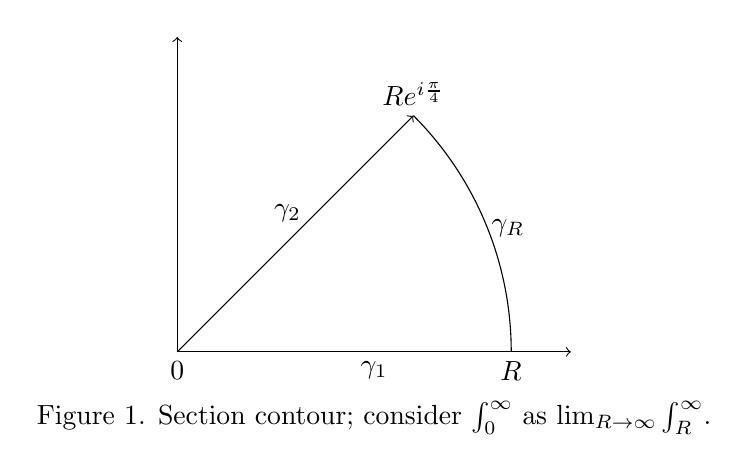
\begin{tikzpicture}[scale=1]
		\draw[->] (0,0) -- (5,0) node[below] {};
		\draw[->] (0,0) -- (0,4) node[left] {};
		\node[below] at (4.24,0) {$R$};
		\node[below] at (0,0) {$0$};
		\node[below] at (2.5,0) {$\gamma_1$};
		\node[below] at (1.4,2.0) {$\gamma_2$};
		\node[below] at (4.2,1.8) {$\gamma_R$};
		\draw[->] (0,0) -- (3,3) node[above] {$Re^{i\frac{\pi}{4}}$};
		\draw (3,3) arc (45:0:4.24);
		\node[below] at (2.5,-0.5) {Figure 1. Section contour; consider $\int_{0}^{\infty}$ as $\lim_{R \to \infty} \int_{R}^{\infty}$.};
	\end{tikzpicture}
\end{figure}
\end{problem}
\begin{proof}
	Since $f(z)=e^{-z^2}$ is a composition of holomorphic functions on $\C$, then $f$ is holomorphic on $\C$.

	Let  $\gamma = \gamma_1 \cup \gamma_R \cup \gamma_2$ be the closed loop section contour in the figure.
	Since $f$ is holomorphic, then it has the closed loop property and $\oint_{\gamma}f\,dz=0$.

	So, we have that \[
		0 = \oint_{\gamma} f\,dz = \int_{\gamma_1} f\,dz + \int_{\gamma_2}f\,dz +  \int_{\gamma_R} f\,dz
		.\]

	But, as $R\to \infty$, $\gamma_1$ parametrizes the positive real line, so \[
		\int_{\gamma_1} e^{-z^2} \,dz = \int_{0}^{\infty} e^{-x^2} \,dx = \frac{\sqrt{\pi} }{2}
	\] because $e^{-x^2}$ is an even function.

	We will show that the integral of $f$ over the arc $\gamma_R$ goes to zero.
	Let $z=re^{i\theta}$.
	On this curve, $r$ is fixed at $R$ and $\theta$ varies from $0$ to  $\frac{\pi}{4}$.

	So, $-z^2 = -R^2e^{2i\theta}$ and $dz=iRe^{i\theta}$.
	Then, \[
		\int_{0}^{\frac{\pi}{4}} iRe^{i\theta} e^{-R^2e^{2i\theta}} \,d\theta
		= \int_{0}^{\frac{\pi}{4}} iRe^{i\theta-R^2e^{2i\theta}} \,d\theta
		.\]

	For $\theta\in \left[0,\frac{\pi}{4}\right]$,
	we have that $e^{2i\theta}\in \left[ e^0, e^{i \frac{\pi}{2}} \right] = [1,i] $.

	So, as $R\to \infty$, we have, \[
		\forall \theta \in \left[ 0, \frac{\pi}{4} \right),\quad\left| Re^{i\theta-R^2e^{2i\theta}} \right| \to 0
		\quad \text{and} \quad
		\theta = \frac{\pi}{4}, \quad \left| Re^{i(\theta-R^2)} \right| \to \infty
		.\]
	However, since the integrand only blows up at a simple point, which has measure zero, then the contribution of this point to the overall integral is zero.
	Hence \[
		\lim_{R \to \infty} \int_{\gamma_R} f \,dz = 0
		.\]

So, maintaining the orientation of each part of the curve $\gamma$, we have that \[
\int_{\gamma_1} f\,dz = -\int_{\gamma_2} f\,dz  
.\] 

	Now, for the integral on the path $\gamma_2$, we fix $\theta=\frac{\pi}{4}$ and vary $r$ from  $0$ to  $R$. 
  Note that this parameterization traverses $\gamma_2$ in the opposite direction of the positively oriented curve $\gamma$, so we will consider the opposite of the resulting integral.

  So, $-z^2=-r^2e^{2i\theta}=-r^2e^{i \frac{\pi}{2}} = -ir^2$ and $dz = e^{i \frac{\pi}{4}}dr = \frac{1}{\sqrt{2} }(1+i) dr$. 

  Then, with the Euler identity, we have that \[
   -\int_{\gamma_2} f\,dz = \frac{1}{\sqrt{2}}(1+i)\int_{0}^{\infty} e^{-ir^2} \,dr = \frac{1}{\sqrt{2} }(1+i) \int_{0}^{\infty} (\cos{r^2}-i\sin{r^2}) \,dr
  .\] 
  With the above equality between the integrals of $\gamma_1$ and $\gamma_2$, we have 
  \begin{align*}
    \frac{\sqrt{\pi}}{2} &= \frac{1}{\sqrt{2} }(1+i) \int_{0}^{\infty} (\cos{r^2}-i\sin{r^2}) \,dr \\
   \sqrt{\frac{\pi}{2}}  &= \int_{0}^{\infty} \cos{x^2} \,dx + \int_{0}^{\infty} \sin{x^2}\,dx + i\left( \int_{0}^{\infty} \cos{x^2}\,dx - \int_{0}^{\infty} \sin{x^2} \,dx \right)  \\
  .\end{align*}
  Considering the real and imaginary parts separately, we have \[
 \int_{0}^{\infty} \cos{x^2}  \,dx  = \int_{0}^{\infty} \sin{x^2}  \,dx
  \] and therefore also \[
  \frac{\sqrt{2\pi}}{4}=\frac{\sqrt{\pi} }{2\sqrt{2} }=\int_{0}^{\infty} \cos{x^2} \,dx = \int_{0}^{\infty} \sin{x^2} \,dx
  \] as desired.
\end{proof}
\end{document}
